\centerline{\bf \Huge Ненаглядная геометрия}

\begin{flushright}
        \scriptsize{Кто первый сдаст все задачи тому тыщу на карту)}
\end{flushright}


\problem{1}
Разрежьте 1-й треугольник на две части и сложите из них 2 -й (см. рис.).

\begin{center}
    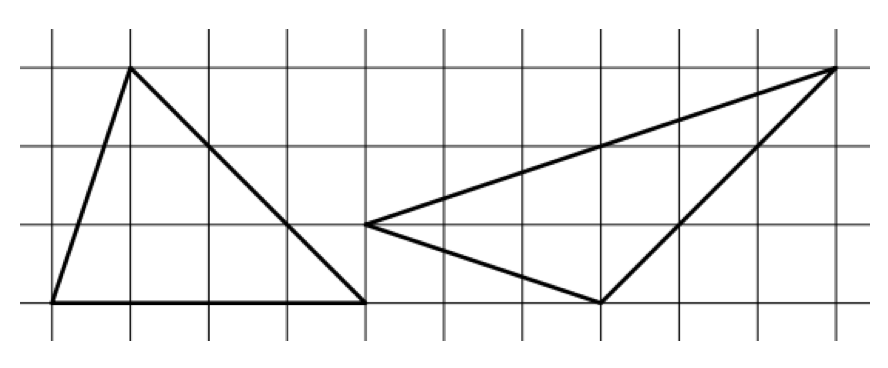
\includegraphics[width=0.4\textwidth]{ЭлМШ 2025-2026/II блок/7/2.3.1.png}
\end{center}

\problem{2}
Прямоугольник $4 \times 9$ произвольно наложили на квадрат $6 \times 6$, как показано на рисунке. Докажите, что площади закрашенных частей прямоугольника и квадрата равны.

\begin{center}
    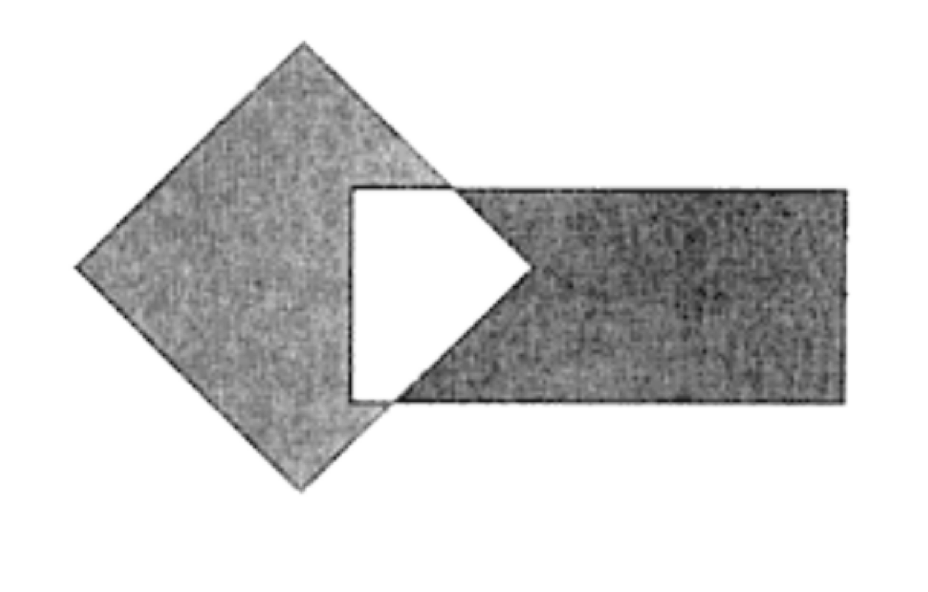
\includegraphics[width=0.4\textwidth]{ЭлМШ 2025-2026/II блок/7/2.3.2.png}
\end{center}

\problem{3}
Три квадрата со сторонами $10 с м, 8 с м, 6 с м$ составили так, как показано на рисунке. Найдите площадь закрашенной фигуры.

\begin{center}
    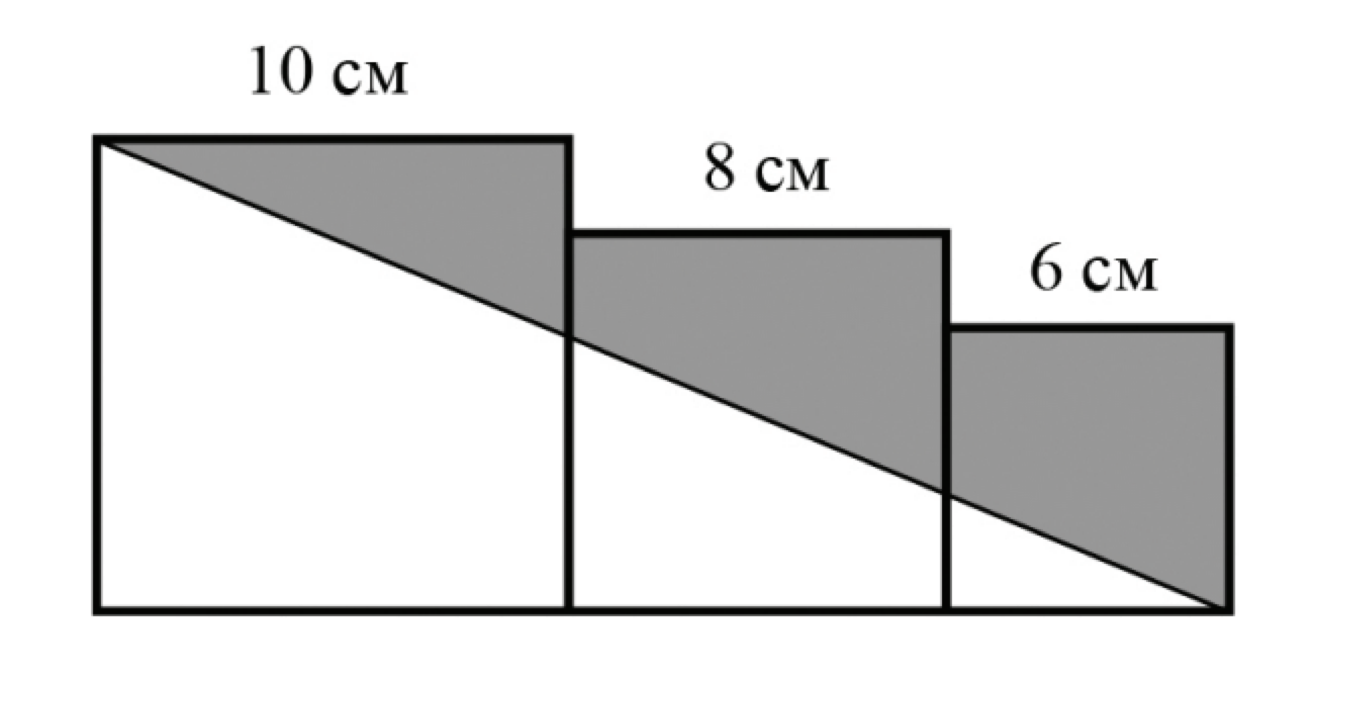
\includegraphics[width=0.4\textwidth]{ЭлМШ 2025-2026/II блок/7/2.3.3.png}
\end{center}

\newpage

\hspace{3mm}

\problem{4}
Прямоугольник $ABCD$ разбит прямыми, проходящими через точку $X$ на 4 прямоугольника (см. рисунок). Докажите, что если $X$ лежит на диагонали $AC$, то площади серых прямоугольников равны.

\begin{center}
    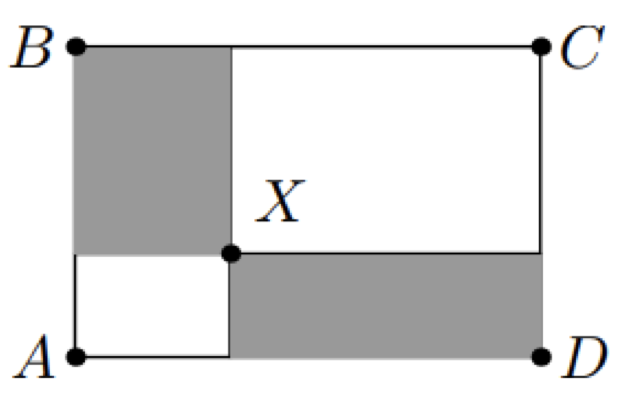
\includegraphics[width=0.4\textwidth]{ЭлМШ 2025-2026/II блок/7/2.3.4.png}
\end{center}

\problem{5}
Лист календаря частично закрыт предыдущим листом (см. рисунок). Какая его часть больше (по площади): открытая или закрытая?

\begin{center}
    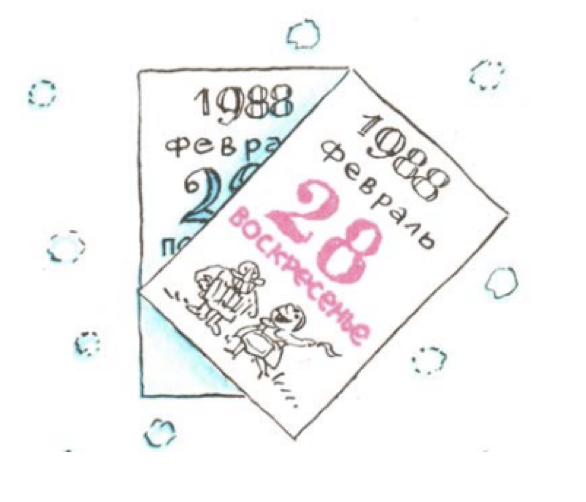
\includegraphics[width=0.4\textwidth]{ЭлМШ 2025-2026/II блок/7/2.3.5.png}
\end{center}